\documentclass[mathserif, aspectratio=169]{beamer}
\usetheme{Warsaw}
\useoutertheme{miniframes}
\useinnertheme{rectangles}
\usecolortheme{albatross}
\usepackage{listings}
\usepackage{pgf}
\usepackage{qtree}
\usepackage{tikz}
\usetikzlibrary{shapes, arrows}
\usepackage{gb4e}

\titlegraphic{
\vspace{1.0em}

\includegraphics[height=1.5em]{images/ucberkeley}
\hfill

\includegraphics[height=1.5em]{images/berkeleylab}
}

\title[Understanding the Aging Process with Artificial Intelligence]{Understanding the Aging Process}
\subtitle{An Automated Approach that Uses Artificial Intelligence}

\author{Mark Farrell}
\institute{

Bioinformatics Researcher \and

Center for Research and Education on Aging \\
Lawrence Berkeley National Laboratory \\
University of California, Berkeley

}

\date{September 4th, 2014}
\subject{Bioinformatics}

\note{
Good afternoon everybody. My name's Mark Farrell and I've been doing research for CREA
remotely from Canada. Today I'd like to inform you about a method I've been working on for
automating the construction of biomedical knowledge bases; specifically a knowledge base on aging.
The presentation should be about 20 minutes in length and there will be an opportunity to ask
questions at the end.
}

\AtBeginSection[]
{
\begin{frame}[plain]
\frametitle{Outline}
\tableofcontents[currentsection]
\end{frame}
}

\lstset{
basicstyle=\small\sffamily,
columns=fullflexible,
showstringspaces=false
}

\noautomath

%\setbeameroption{show notes}
\setbeamercolor{note page}{bg=white!90!black, fg=black}

\begin{document}

\begin{frame}[plain]
\titlepage
\end{frame}

\section{About Me}

\begin{frame}

\frametitle{Who I am}
\framesubtitle{Mark Farrell}

\centering

\begin{tabular}{c c}
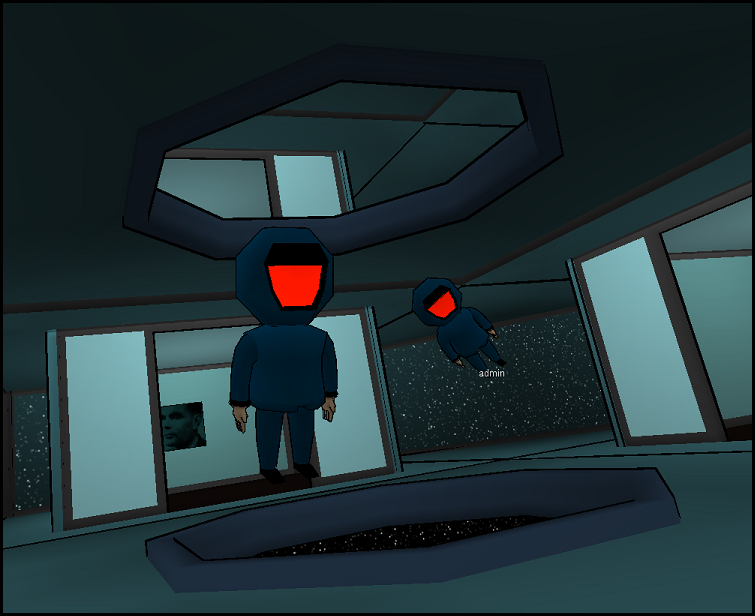
\includegraphics[width=.2\linewidth]{images/starfall.png}&
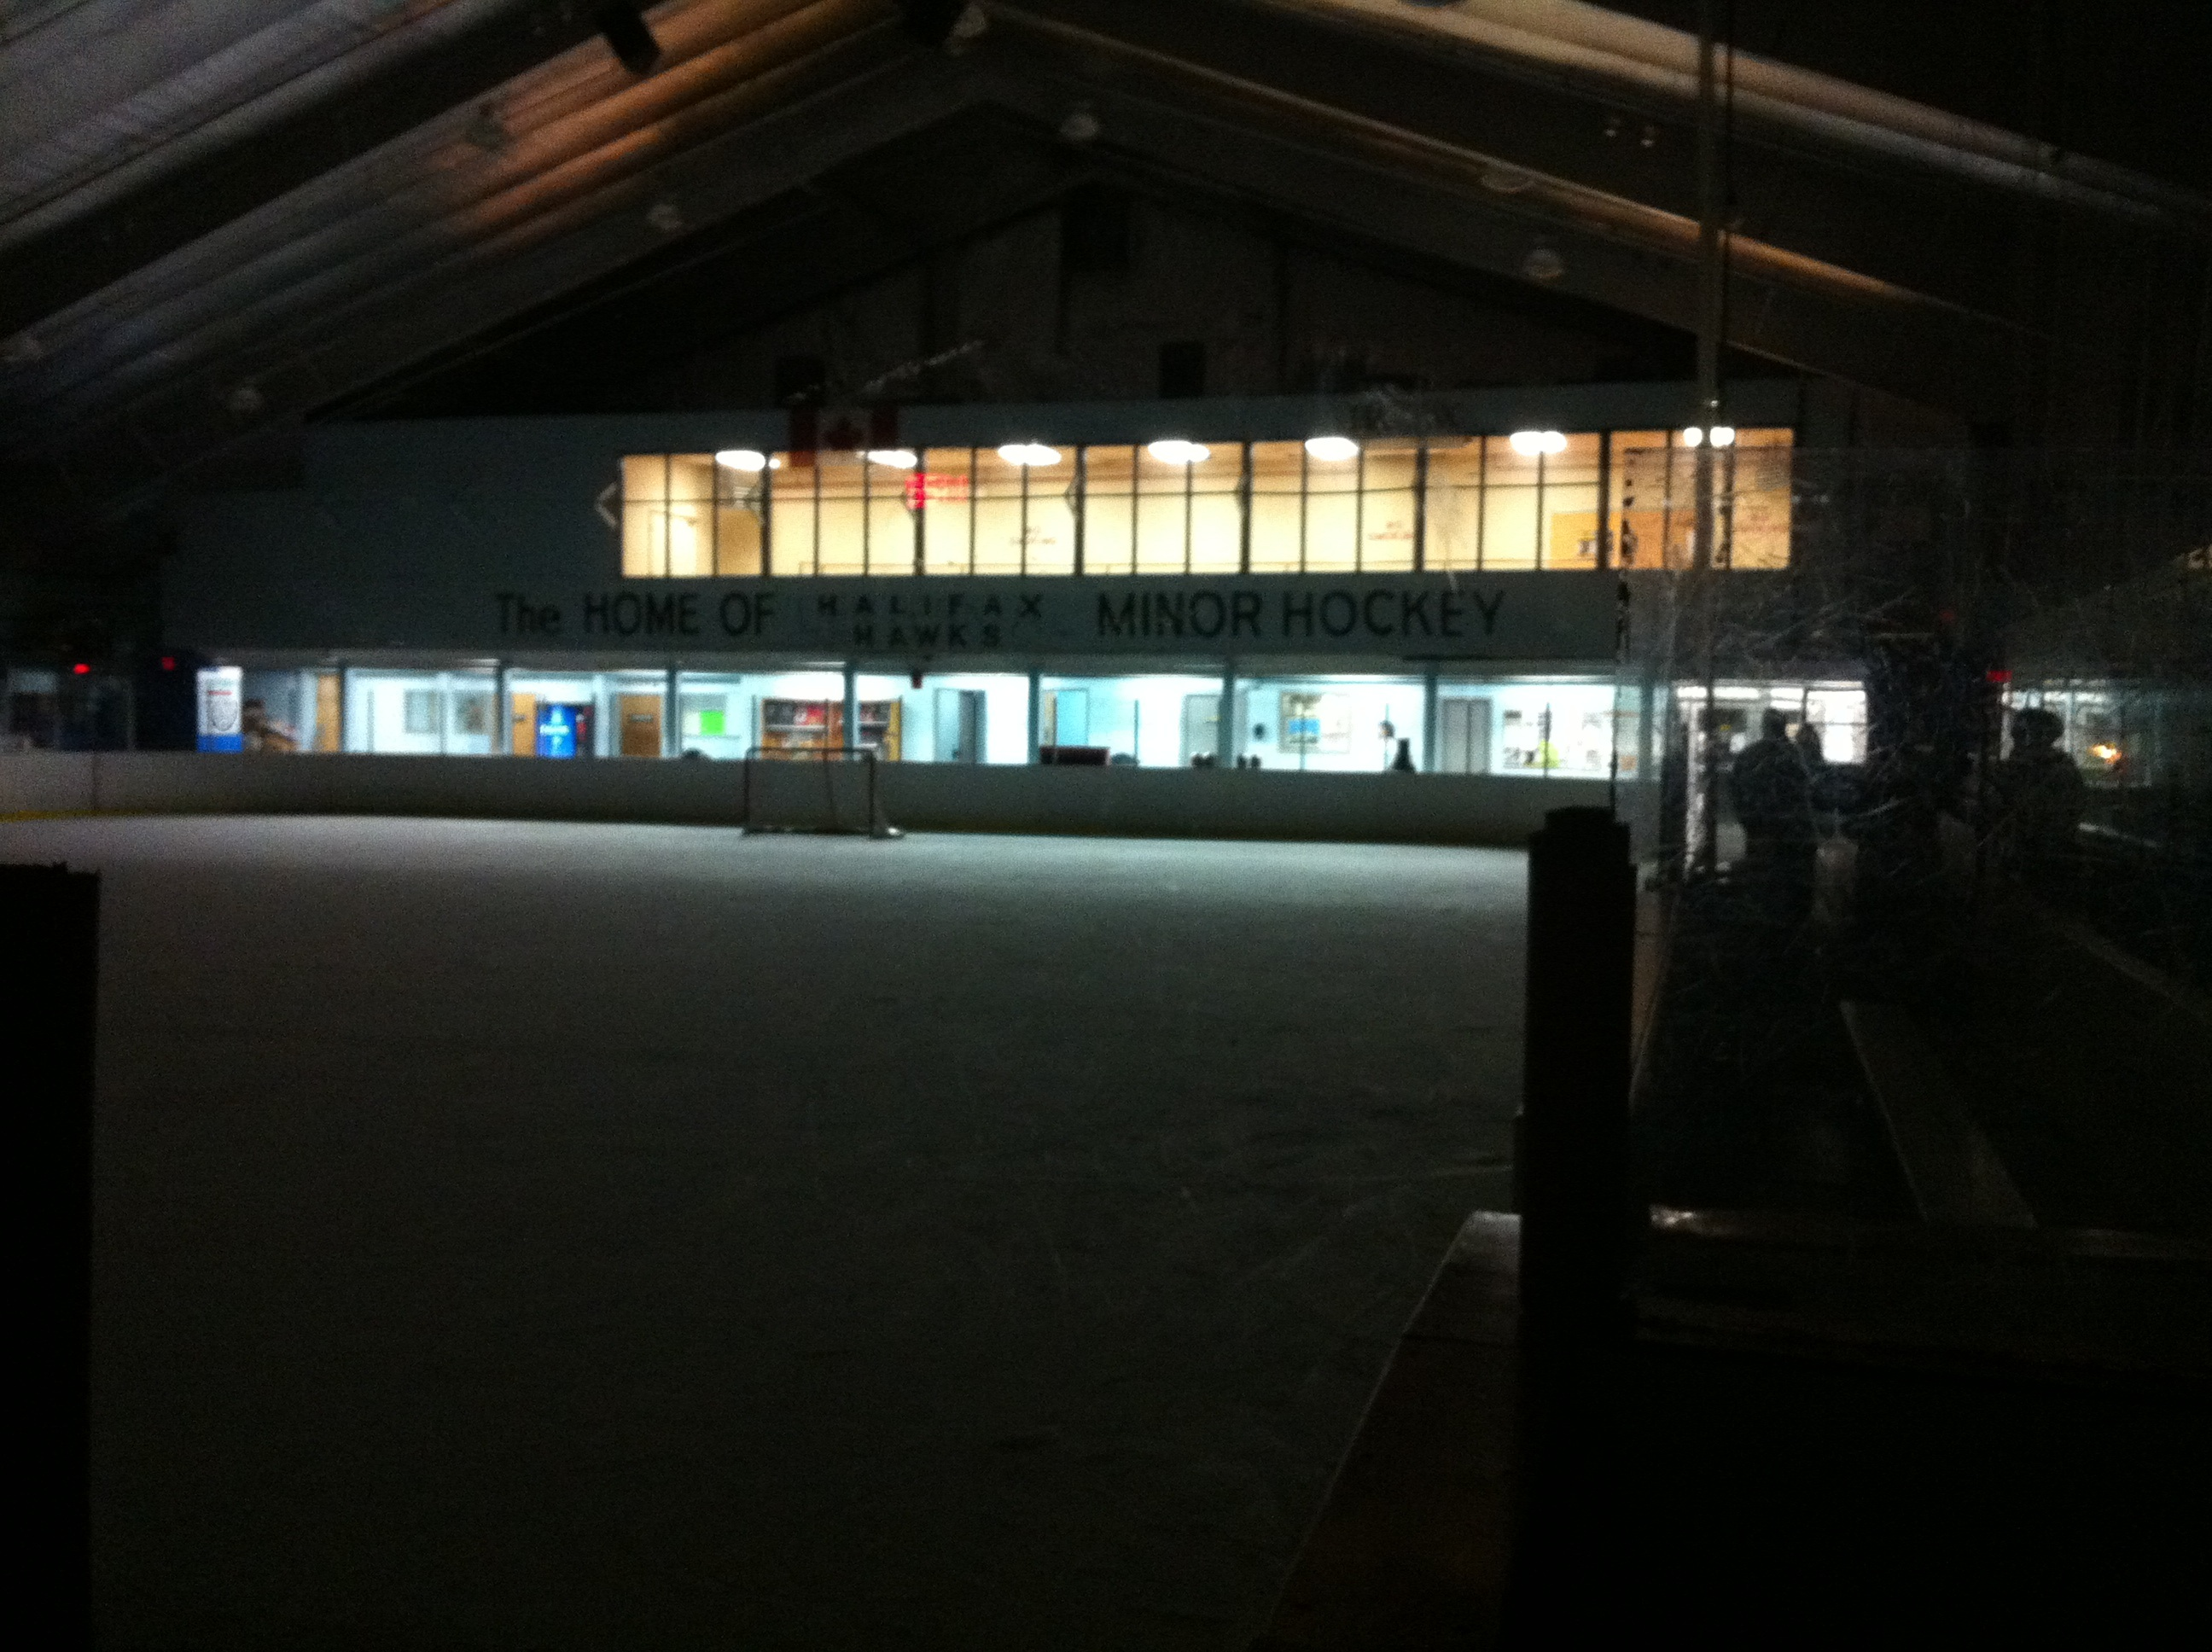
\includegraphics[width=.2\linewidth]{images/rink.jpg}\\
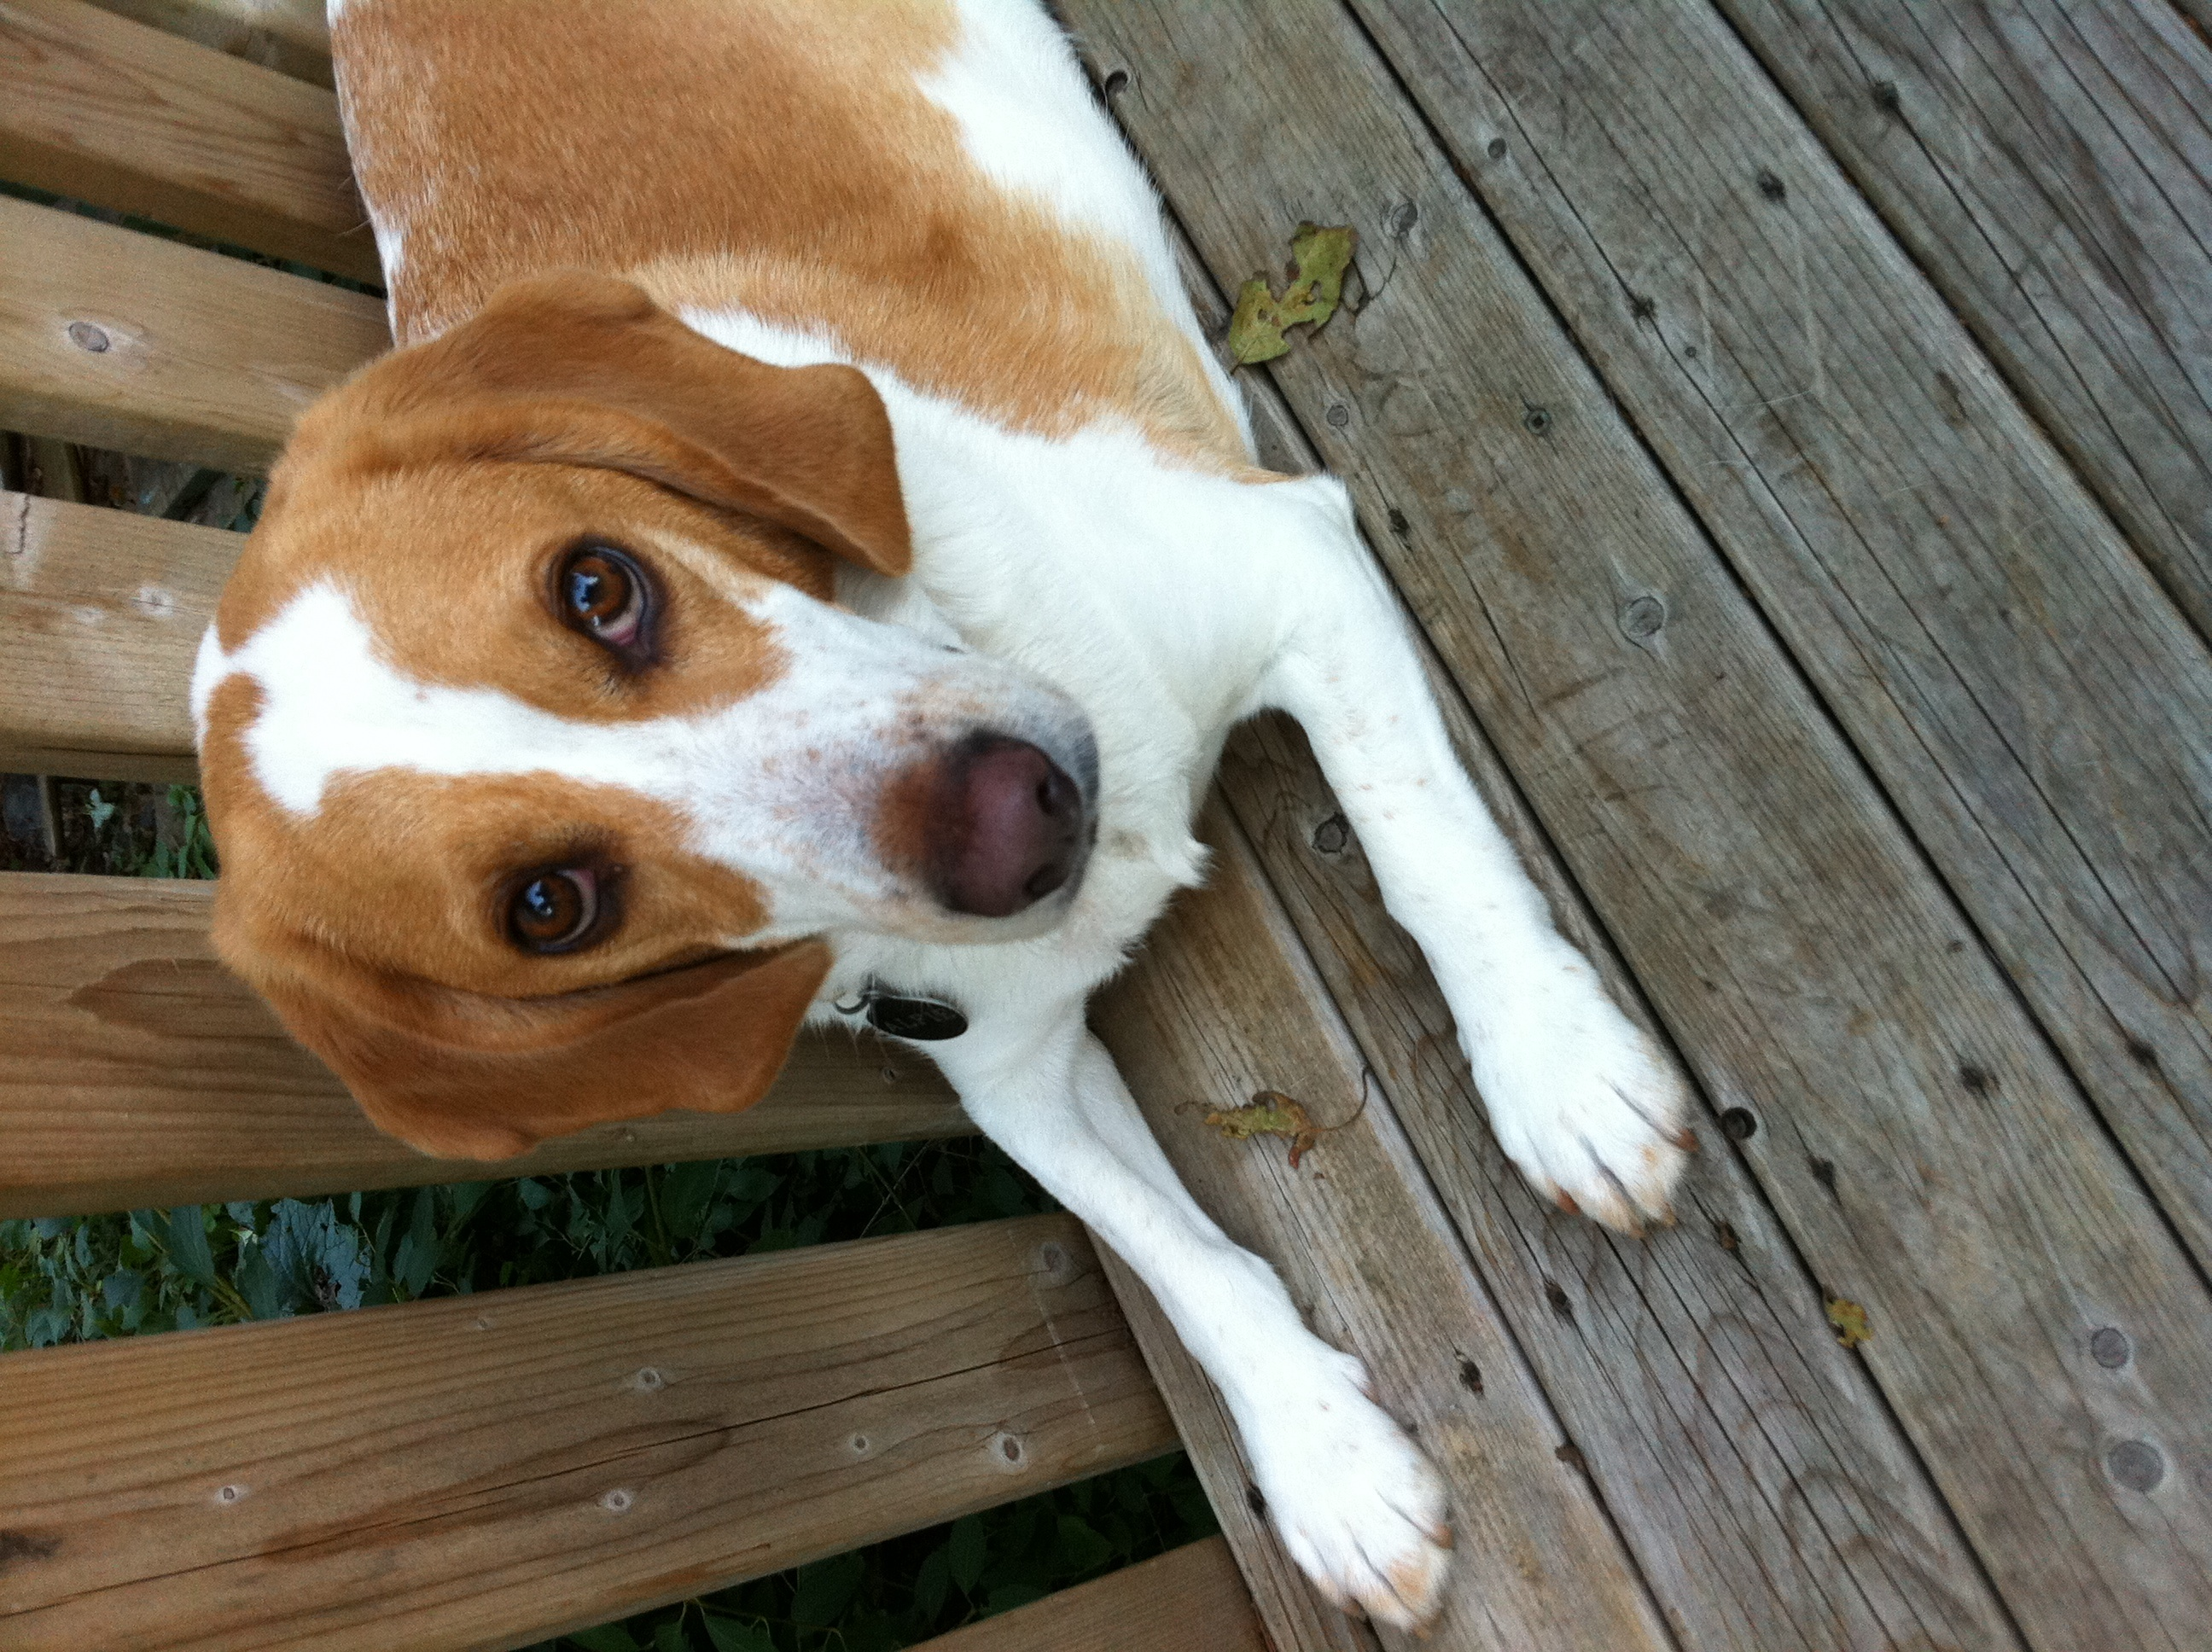
\includegraphics[angle=270, origin=c, width=.2\linewidth]{images/alfie.jpg}&
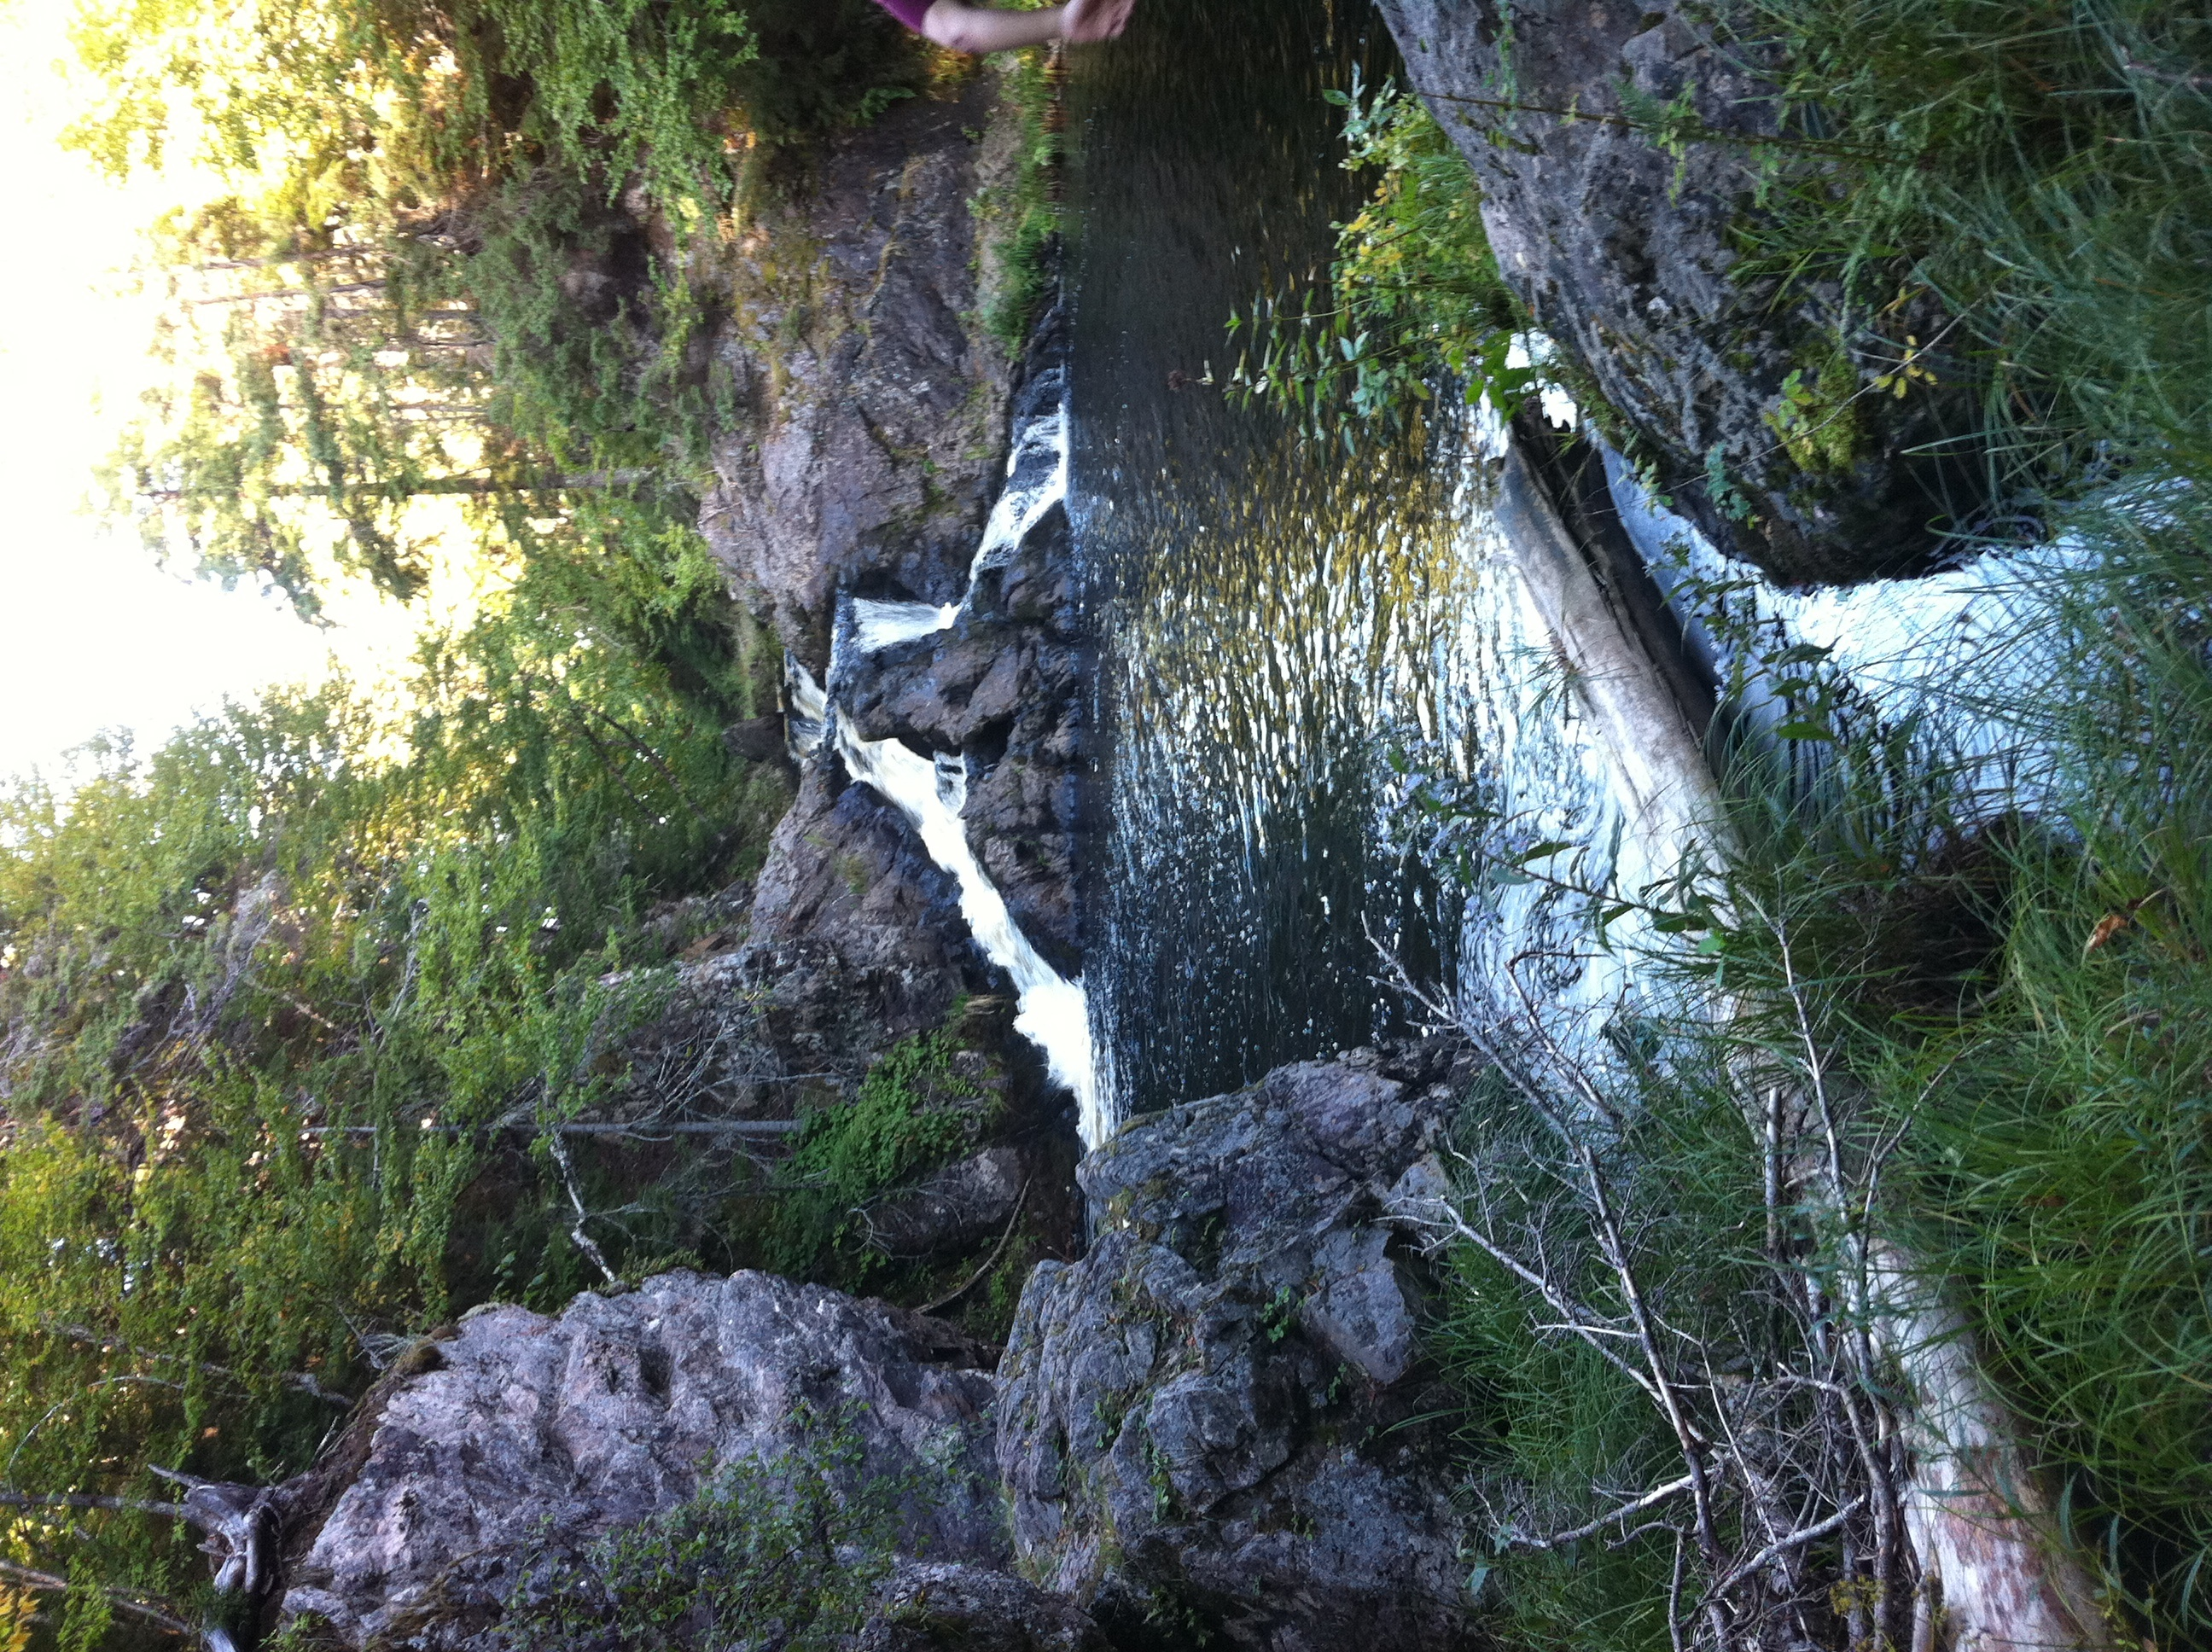
\includegraphics[angle=270, origin=c, width=.2\linewidth]{images/camping.jpg}
\end{tabular}

\end{frame}

\note{
This is my first time being here in person, so I doubt many of you know who I am.
So, I'm going to start off by introducing myself.
}

\begin{frame}
\frametitle{Where I'm from}
\framesubtitle{Atlantic Canada}
\centering
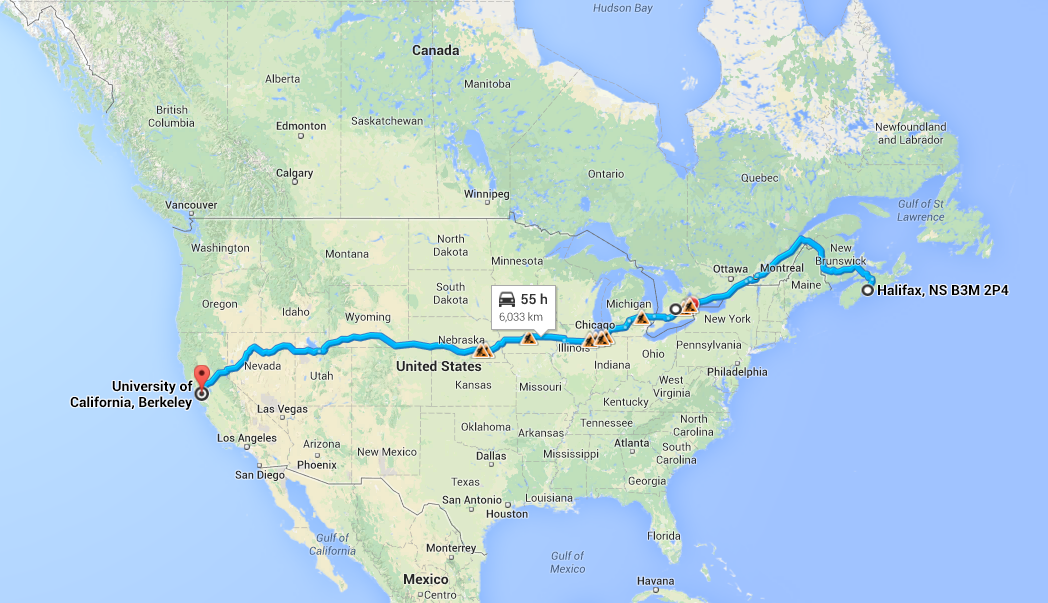
\includegraphics[height=.75\textheight]{images/map.png}
\end{frame}

\note{
I grew up on Canada's East Coast, and was back home again this summer.
So, I've had to travel quite a bit over the past few days in order to arrive here at Berkeley.
}

\begin{frame}

\frametitle{What I'm Studying}

\begin{columns}
\begin{column}{.7\textwidth}
\begin{description}
\item[Year] 2
\item[Program] Bachelor of Computer Science
\item[Faculty] Mathematics
\item[Institution] University of Waterloo
\item[Location] Waterloo, Ontario, Canada
\end{description}
\end{column}
\begin{column}{.3\textwidth}
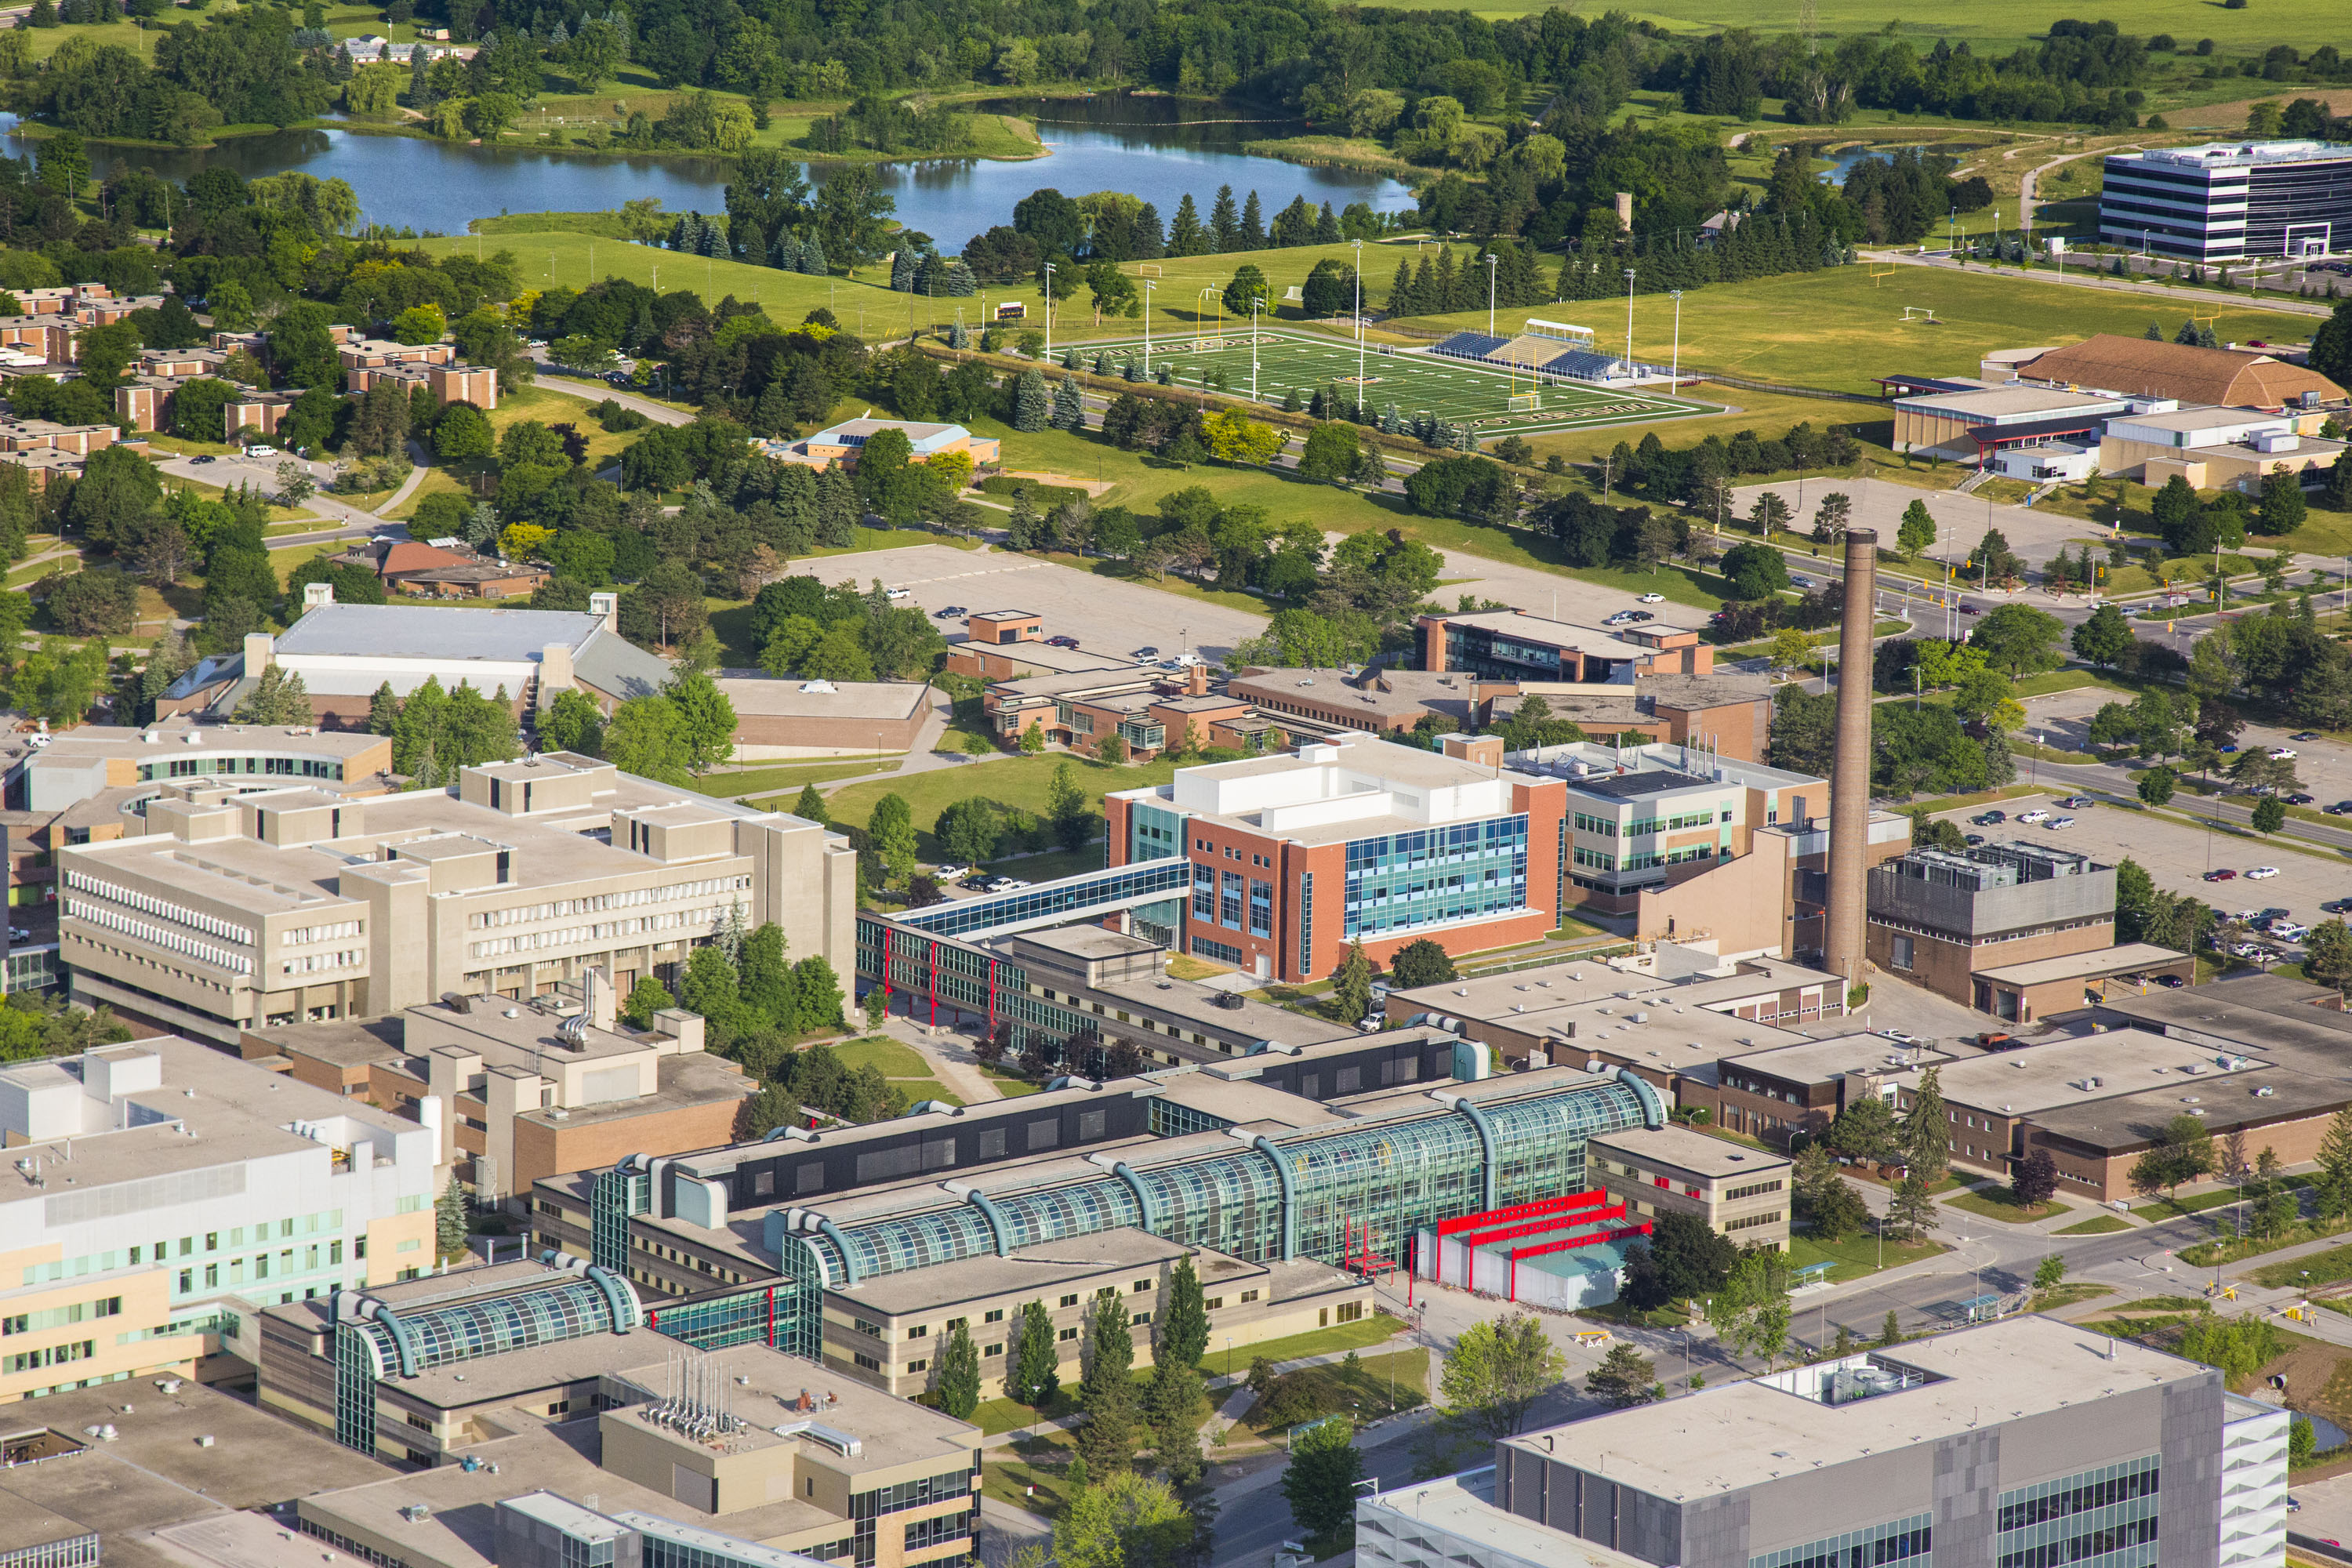
\includegraphics[width=1.0\linewidth]{images/campus.jpg}
\end{column}
\end{columns}

\end{frame}

\note{
And in case you're wondering, I'm going into my second year of undergraduate studies
at the University of Waterloo, majoring in Computer Science.
}

\begin{frame}

\frametitle{How I Became a Researcher at CREA}
\framesubtitle{Prof. Garan Emailed the University of Waterloo Computer Science Club}

\centering

\begin{tabular}{c c}
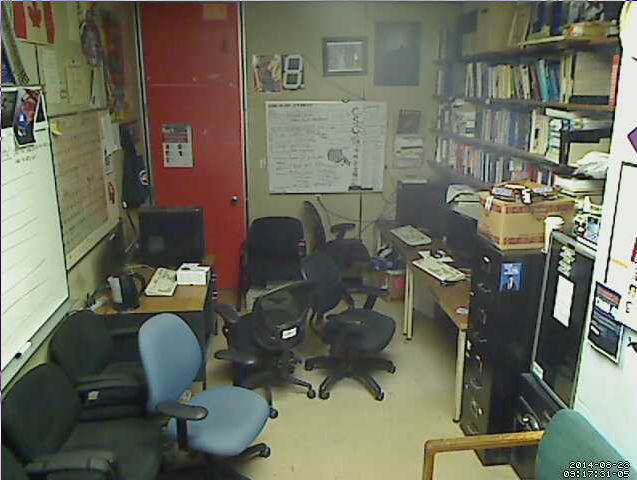
\includegraphics[width=0.30\linewidth]{images/malto_webcam.png} &
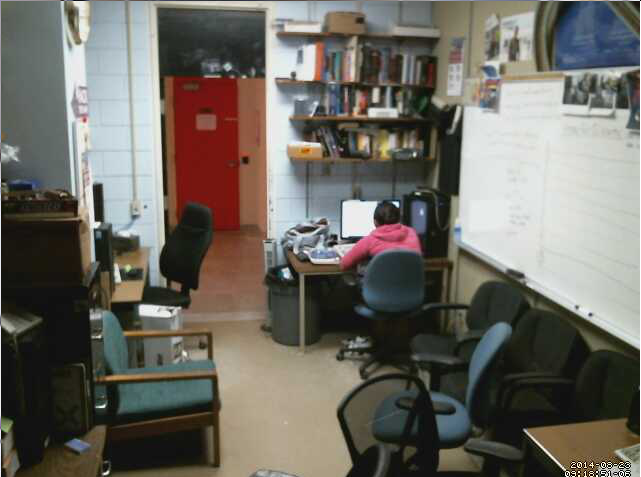
\includegraphics[width=0.30\linewidth]{images/bitshift_webcam.png}\\

\includegraphics[width=0.30\linewidth]{images/csc.png} &
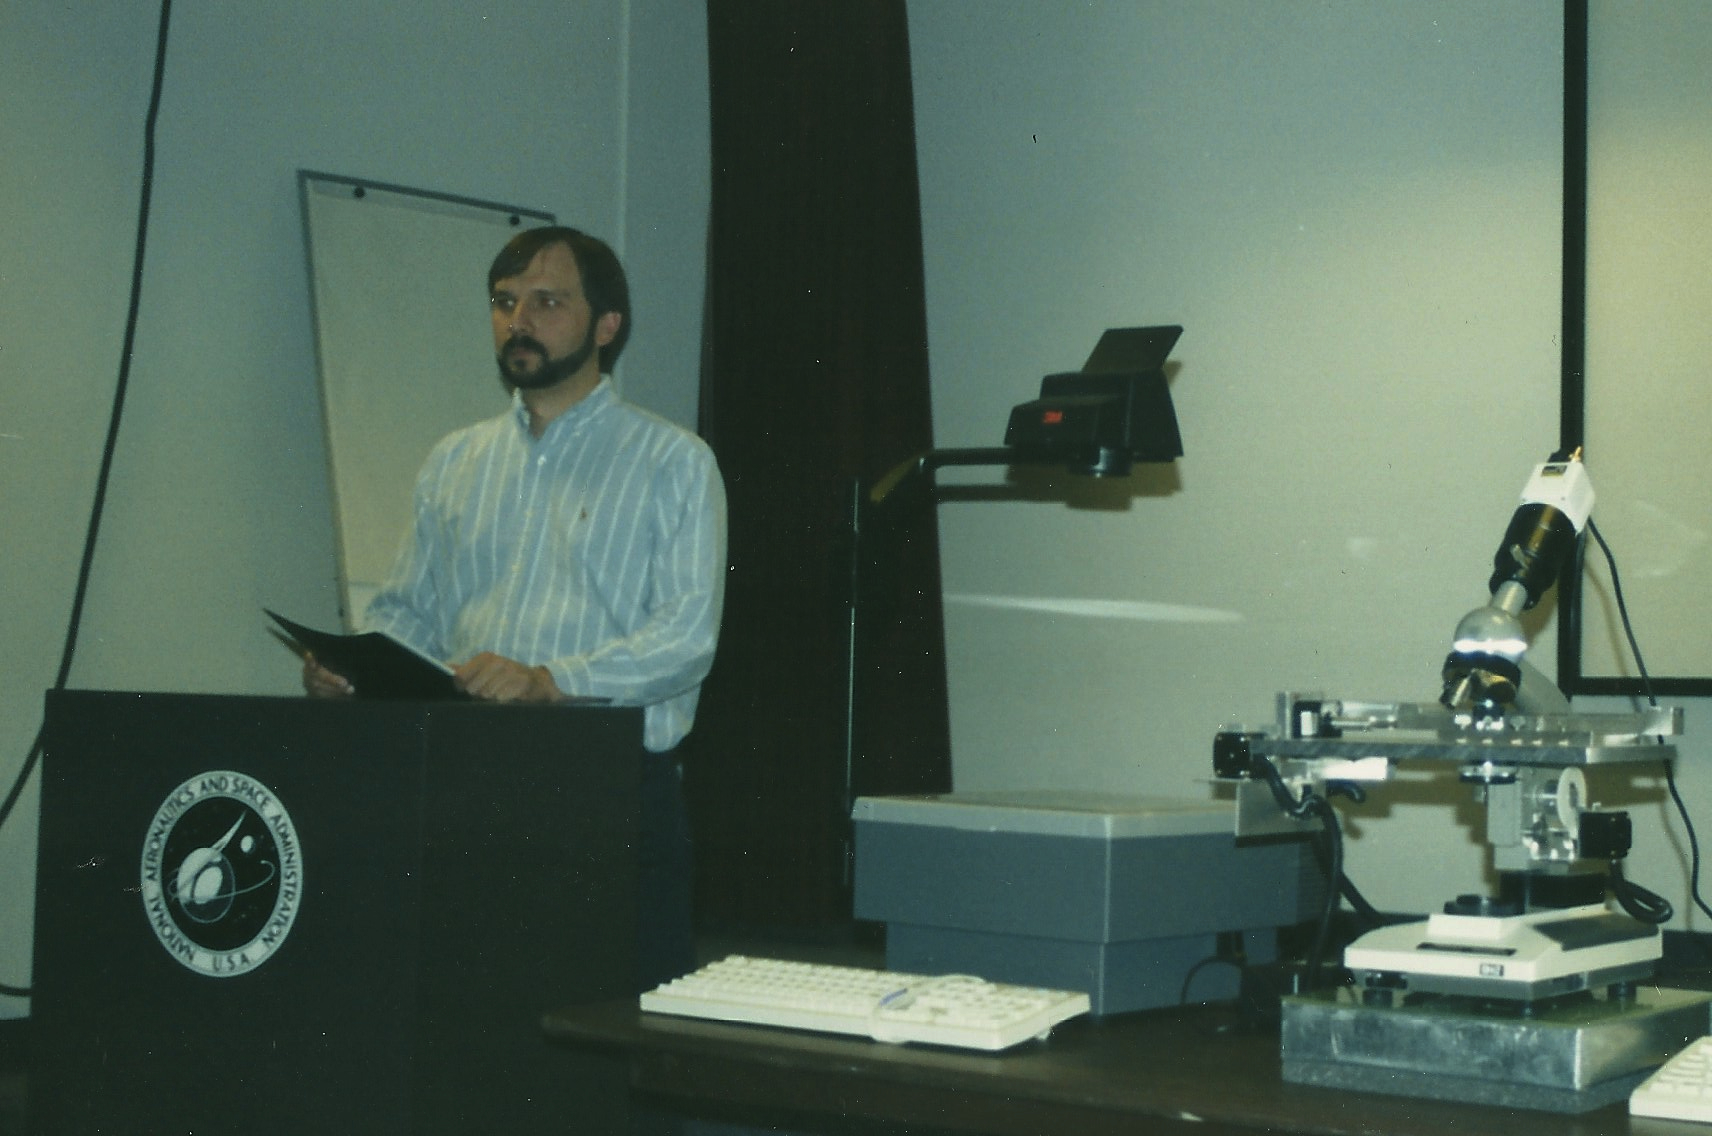
\includegraphics[width=0.30\linewidth]{images/steve_garan.jpg}\\
\end{tabular}

\end{frame}

\note{
That's all very well and good: I haven't explained how I got involved
with research at CREA. Steve Garan (you might know him) emailed the University of Waterloo
Computer Science Club back in January, looking for
current members interested in an AI internship; he used to
be President back in the 80s. It looked interesting, so I began working
with him, meeting weekly on Skype to discuss progress.
}

\begin{frame}

\frametitle{Why was I Interested in Research at CREA?}

\centering
\begin{tabular}{ c | c }
Hobby & CREA Research \\
\hline
Reverse Engineering & Natural Language Processing\\
Game Development & Artificial Intelligence\\
Health & Bioinformatics\\
\end{tabular}

\end{frame}

\note{
So, why was I interested in research at CREA? I've worked on some
software projects involving reverse engineering network protocols and
game development in my spare time. And, I felt that CREA was offering me an
opportunity to hone my interests, allowing me to deepen my knowledge of computing
beyond what I would likely accomplish on my own.
}

\section{Understanding the Aging Process}

\note{
Ok, so let's talk about 'Understanding Aging' and where I come in.
}

\begin{frame}

\frametitle{What does CREA want to do?}
\framesubtitle{CREA Wants to Understand Aging and Increase Human Lifespan}

\centering

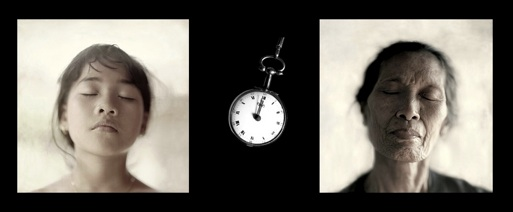
\includegraphics[height=.5\textheight]{images/aging}

\end{frame}

\note{
As you might already know, CREA wants to understand aging and increase
human lifespan.
}

\begin{frame}

\frametitle{Why is it Difficult to Understand Aging?}

\centering
\only<1>{

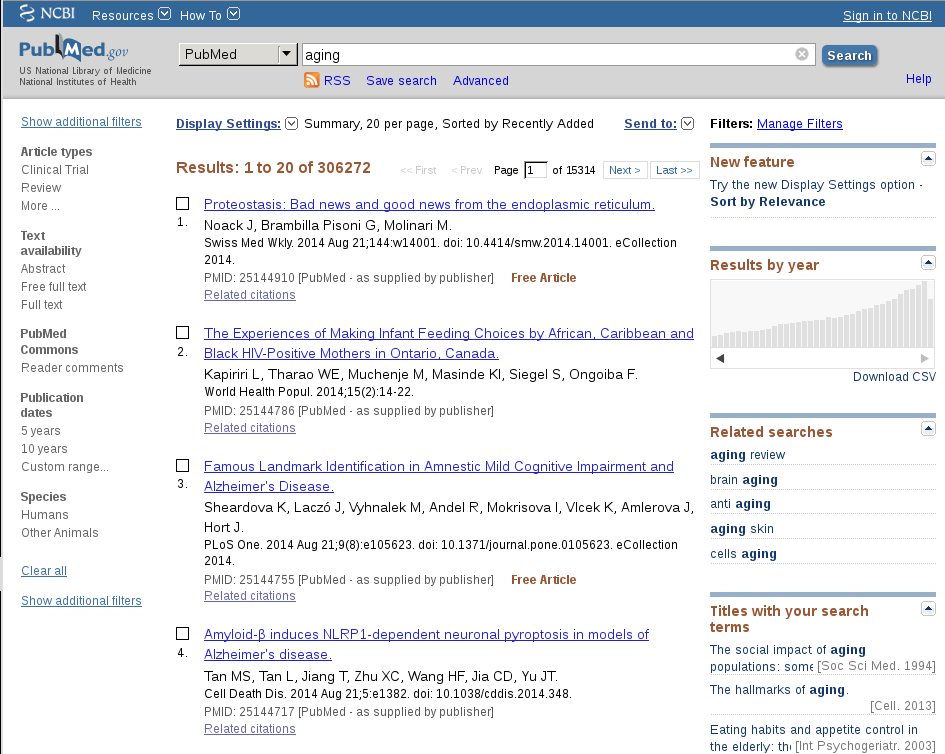
\includegraphics[width=.95\textheight]{images/pubmed}

\note{
But, Why is it Difficult to Understand Aging?
If you look at this figure here, you can see that not only is there a large
volume of publications made on the subject, but also the
rate at which new publications are being made has been doubling over the past few
decades.
}

}

\only<2>{

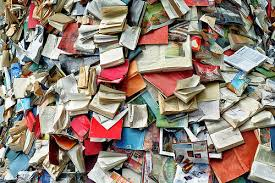
\includegraphics[width=.5\linewidth]{images/cascadeofbooks.jpg}

\note{
So, we need a better way to manage past and future knowledge that will help us understand
aging; this is a problem.
}

}

\end{frame}

\begin{frame}

\frametitle{How can CREA Understand Aging?}
\framesubtitle{Build a Knowledge Base that Describes and Reasons about Aging}

\centering

\only<1>{

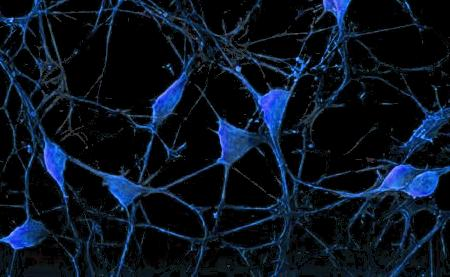
\includegraphics[height=.75\textheight]{images/knowledgebase.jpg}

\note{
And that's where I come in. I've been trying to work on a solution to this problem, which
involves building a knowledge base, software, that can assist humans in order to understand
aging and develop theories about it.
}

}

\only<2>{

\tikzstyle{decision} = [diamond, draw, fill=blue!60,
text width=4.5em, text badly centered, node distance=2.5cm, inner sep=0pt]
\tikzstyle{block} = [rectangle, draw, fill=blue!60,
text width=5em, text centered, rounded corners, minimum height=4em]
\tikzstyle{line} = [draw, -latex']
\tikzstyle{cloud} = [draw, ellipse,fill=red!60, node distance=3cm,
minimum height=2em]

\begin{tikzpicture}[scale=1, node distance = 2cm, auto]
\node [block] (acquire) {Acquire Biomedical Articles};
\node [block, below of=acquire] (extract) {Extract Knowledge};
\node [cloud, right of=acquire] (machine) {Machine};
\node [cloud, left of=acquire, node distance=4cm] (human) {Human};
\node [block, below of=human] (gui) {Graphical User Interface};
\node [decision, below of=extract] (belongs) {Is about Aging?};
\node [block, left of=belongs, node distance=4cm] (update) {Update Aging Theory};
\node [block, right of=belongs, node distance=4cm] (discard) {Discard};
\path [line] (acquire) -- (extract);
\path [line, dashed] (machine) -- (acquire);
\path [line, dashed] (extract) -| (machine);
\path [line] (extract) -- (belongs);
\path [line] (belongs) -- node{yes}(update);
\path [line] (belongs) -- node{no}(discard);
\path [line, dashed] (human) -- (acquire);
\path [line, dashed] (human) -- (gui);
\path [line] (gui) -- (update);
\end{tikzpicture}

\note{
Have a look at this figure: the idea behind the software project I'm working on is to get a machine
to read text and try to understand aging, just like how human's can try understand to aging by
reading texts and journal articles. And also, to present a machine's understanding of aging to humans
and allow them correct and modify the machine's understanding of aging in an intuitive way.
}

}

\end{frame}

\section{Knowledge Extraction}

\note{
To date, I've made quite a bit of progress in allowing a machine to read and extract knowledge from
text articles, and have also been able to display that knowledge in a manner that helps humans understand aging.
However, I haven't made much progress on allowing the machine to form a theory of aging and reason about aging
itself; i.e. it can't really decide what knowledge is relevant to aging and what it is not.
}

\begin{frame}

\frametitle{Knowledge Extraction}
\framesubtitle{Overview of Progress}

\centering

\begin{block}{Input}
... The \textcolor{orange}{pyridinoline} and \textcolor{orange}{desmosine}
were \textcolor{pink}{examined} as \textcolor{orange}{candidate sensitizer chromophores}
\textcolor{pink}{contained} in \textcolor{orange}{collagen} and \textcolor{orange}{elastin},
respectively. ...
\end{block}

\begin{block}{Output}
\centering
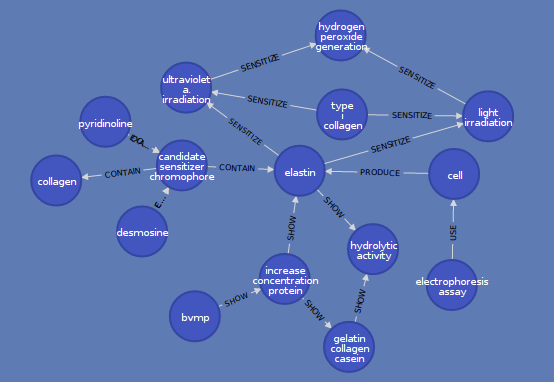
\includegraphics[height=.4\textheight]{images/elastinneighborhood}
\end{block}

\note{
As Steve Garan put it, aging can be looked at as the degradation over
time and eventual failure of an organism's systems. So let's start off
talking about knowledge extraction with an excerpt from a journal abstract
that is related to elastin degradation. Have a look at the example input sentence:
I've highlighted the literal nouns found in the sentence and the literal verbs that
relate nouns to one another. Now look at the output: knowledge extraction is the process
of identifying literal nouns and relating them to each other, i.e. making logical assertions
about the actions that they can perform on one another.
}

\end{frame}

\note{
Natural language data is rather unstructured,
and so I have to decide on what components of natural language are essential for describing how
systems and processes work when translating it into a structured format that a machine can understand
and reason about. There are problems with the same literal nouns and verbs being used to represent
multiple concepts in natural language. Take people's names for example: i.e. two different people
can have the same name. However, I need to be able to blindly extract knowledge first before
worrying about those problems, and extracting knowledge blindly is still quite useful for us when
it comes to understanding and reasoning about aging; we just have to be aware that there could be
problems.
}

\begin{frame}

\frametitle{Knowledge Extraction}
\framesubtitle{Method}

\begin{description}

\item[Tokenization] Input a text document and read it, one sentence at a time.
\item[Parsing] For each sentence, generate a constituent tree that describes its phrase structure.
\item[Compilation] Extract facts by pattern matching on each constituent tree.

\end{description}

\end{frame}

\note{
And this is how my software extracts knowledge from text articles. Read the sentences left to
right, one at a time, and extract knowledge from each sentence. Examine the grammatical structure of
each sentence and translate it into a format that a machine can understand and reason about; that's knowledge
extraction.
}

\begin{frame}

\frametitle{Constituent Tree Tags}
\framesubtitle{Word Level}

\centering

\begin{tabular}{c | c | c}
Tag & Meaning & Example \\
\hline
DT & Determiner & the \\
IN & Preposition & of\\
JJ & Adjective & blue\\
RB & Adverb & quickly\\
CC & Coordinating Conjunction & and \\
NN & Singular Noun & monkey\\
NNS & Plural Noun & monkeys\\
VB & Base Verb & fall\\
VBZ & Singular Present Verb & falls\\
VBD & Past Tense Verb & fell\\
VBN & Past Participle Verb & fallen\\
VBG & Gerund Verb & falling\\
... & ... & ...\\
\end{tabular}

\end{frame}

\note{
But, there needs to be some way for a machine to examine sentence structure. Let's first
talk about how linguists might formally examine sentence structure, so that it becomes obvious
how a machine might do so as well. First, they'd label what part-of-speech each word is in a sentence: e.g.
"blue" is an adjective, "dog" is a singular noun and so on and so forth.
}

\begin{frame}

\frametitle{Constituent Tree Tags}
\framesubtitle{Phrase Level}

\centering

\begin{tabular}{c | c | c}
Tag & Meaning & Example \\
\hline
NP & Noun Phrase & the woman \\
VP & Verb Phrase & calls the man \\
PP & Prepositional Phrase & from the store \\
ADVP & Adverb Phrase & quickly and quietly \\
ADJP & Adjective Phrase & blue and red \\
CONJP & Conjunctive Phrase & as well as \\
... & ... & ...\\
\end{tabular}

\end{frame}

\note{
Then, they'd label groups of words that contain certains parts-of-speech - these are called phrases.
For example "the woman" is a phrase, containing a determiner and singular noun.
}

\begin{frame}

\frametitle{Constituent Tree Tags}
\framesubtitle{Clause Level}

\centering

\begin{tabular}{c | c | c}
Tag & Meaning & Example \\
\hline
S & Declarative Clause & the dog walks\\
SBAR & Conjunction + Clause & that the dog walks\\
... & ... & ...\\
\end{tabular}

\end{frame}

\note{
And lastly, groups of phrases that, together, form a logical proposition, are called clauses.
For instance "the dog walks" is a clause because, when read, it makes a logical assertion about
the dog.
}

\begin{frame}

\frametitle{Knowledge Extraction}
\framesubtitle{Example}

\only<1>{
\begin{block}{Input Token}
The man walks the dog.
\end{block}

\note{
Now let's look at this example sentence and its grammatical structure.
}

}

\only<2>{
\begin{block}{Parse Token}
\small
\Tree [.ROOT [.S [.@S [.NP [.DT The ] [.NN man ] ] [.VP [.VBZ walks ] [.NP [.DT the ] [.NN dog ] ] ] ] [.. ] ] ]
\end{block}

\note{
Based on the information I just gave you, we could have created this illustration of
the sentence's structure ourselves. But, a machine needs to be able to do this as well,
it needs to be able to parse sentences and generate constituent trees, in order to
extract knowledge from them. So, there are several software tools available for training a machine
to parse sentences, some using different methods than others; I have been using software called The
Berkeley Parser, which worked fairly well, i.e. it has been fairly accurate when parsing sentences.
}

}

\only<3>{
\begin{block}{Compile Token}
\small
\Tree [.ROOT [.S [.@S [.NP [.DT The ] [.NN man ] ] [.$\langle$predicate:walk$\rangle$ [.NP [.DT the ] [.NN dog ] ] ] ] [.. ] ] ]
\end{block}
}

\only<4>{
\begin{block}{Compile Token}
\Tree [.ROOT [.$\langle$predicate:walk$\rangle$ [.NP [.DT The ] [.NN man ] ] [.NP [.DT the ] [.NN dog ] ] ] ]
\end{block}
}

\only<5>{
\begin{block}{Compile Token}
\Tree [.ROOT [.$\langle$predicate:walk$\rangle$ $\langle$argument:man$\rangle$ $\langle$argument:dog$\rangle$ ] ]
\end{block}
}

\only<6>{
\begin{block}{Output Fact}
\centering
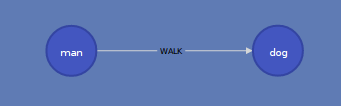
\includegraphics[width=.5\linewidth]{images/manwalkdog.png}
\end{block}
}

\end{frame}

\begin{frame}

\frametitle{Software Demonstration}
\framesubtitle{A preview of CREA's knowledge base, compiled from PubMed abstracts.}

\centering
\href{http://markfarrell.ca/creal}{
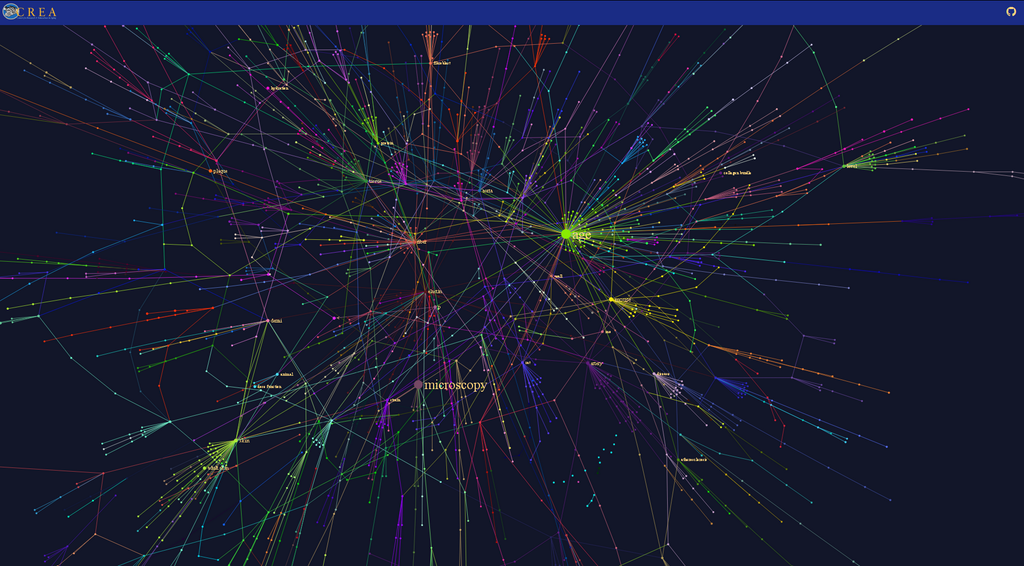
\includegraphics[height=.75\textheight]{images/results}
}

\end{frame}

\begin{frame}

\frametitle{High Performance}
\framesubtitle{Knowledge can be extracted from many sentences at the same time.}

\centering

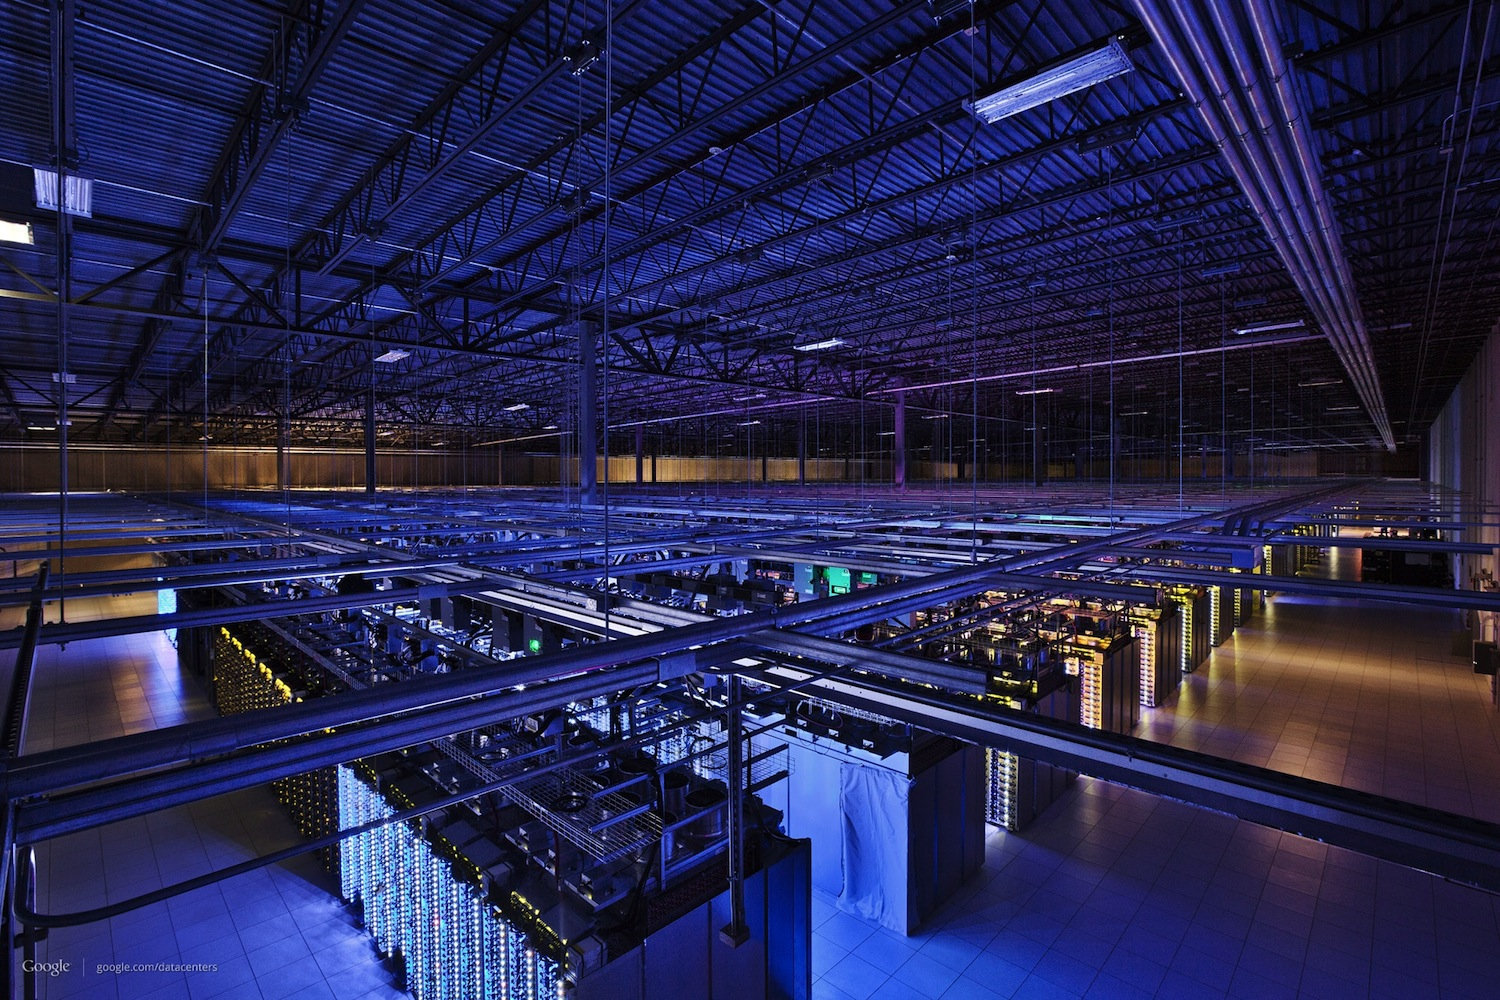
\includegraphics[height=.75\textheight]{images/parallel.jpg}

\end{frame}

\section{What Next?}

\begin{frame}

\frametitle{What Next?}

\centering

\begin{tabular}{c | c}
Task &  Assignees\\
\hline
\textcolor{green}{Research Direction} & \textcolor{green}{Steve Garan} \\
\textcolor{yellow}{Knowledge Extraction} & \textcolor{yellow}{Mark Farrell} \\
\textcolor{yellow}{Text Article Retrieval} & \textcolor{yellow}{Grace Park, Jeremy Wan} \\
\textcolor{yellow}{Knowledge Visualization} & \textcolor{yellow}{Mark Farrell} \\
\textcolor{orange}{Graphical User Interface} & \textcolor{orange}{Mark Farrell} \\
\textcolor{red}{Biomedical Spam Filtering} & \textcolor{red}{---} \\
\textcolor{red}{Automated Reasoning} & \textcolor{red}{---} \\
\end{tabular}

\end{frame}

\begin{frame}

\frametitle{Get Involved}
\framesubtitle{Contact Me for More Information}

\begin{description}
\item[Email] m4farrel@csclub.uwaterloo.ca
\item[Website] markfarrell.ca
\end{description}

\end{frame}

\begin{frame}[plain]
\centering
Questions?
\end{frame}

\end{document}
